\section{Evaluation}
\label{sec:evaluation}

We evaluate \sys around four research questions:

\begin{itemize}
  \item[\textit{RQ1}] \textit{(Problem evidence)} Do real embodied AI projects contain evaluation deviations and evaluation-affecting factors that justify a dedicated diagnosis task?
  \item[\textit{RQ2}] \textit{(Status classification)} Can \sys distinguish setup-sensitive deviations, likely true regressions, and unknown evidence states?
  \item[\textit{RQ3}] \textit{(Factor attribution and abstention)} When a deviation is detected, can \sys identify the responsible engineering factor, and can it abstain on non-deviating calibration cases?
  \item[\textit{RQ4}] \textit{(Diagnosis cost)} How much execution cost does factor-directed diagnosis require relative to the evidence it provides?
\end{itemize}

\subsection{Experimental Setup}
\label{sub:eval-setup}

\noindent\textbf{Benchmark stack.} The controlled experiments use LeRobot+LIBERO with the \mbox{\emph{pi0\_libero\_finetuned\_v044}} policy. A case consists of a baseline run, a current run, and zero or more replay runs. Each completed-run artifact records \mbox{\emph{manifest.json}}, \mbox{\emph{episodes.jsonl}}, \mbox{\emph{summary.json}}, and \mbox{\emph{logs.txt}}. Failed-run artifacts additionally record \mbox{\emph{failure.json}}. This artifact interface is important because \sys is not allowed to infer a factor from prose notes alone: every diagnosis must trace to structured artifacts, replay evidence, or a declared missing-evidence condition.

\noindent\textbf{Ground-truth isolation.} The cases are controlled, but the evaluator and the diagnosis engine use different information. Case configurations contain expected factors for scoring, while \sys consumes only baseline/current/replay artifacts. The aggregation scripts compare the produced diagnosis against the expected factor after the report is written. This separation matters because otherwise a controlled case would risk testing whether the system can read an injected label rather than whether it can diagnose from behavior and replay evidence.

\noindent\textbf{Realism and control.} The controlled cases are not toy outputs or synthetic summaries. Each case executes the LeRobot+LIBERO stack and writes the same artifact contract used by the diagnosis pipeline. Control enters at the factor level: we choose one evaluation-affecting change, run the corresponding baseline/current/replay artifacts, and then check whether the diagnosis recovers the expected factor from artifacts alone. This design gives the experiment a causal oracle without relying on naturally occurring histories whose true cause may be undocumented. RQ1 supplies the empirical evidence that such symptoms and factors occur in real projects; RQ2--RQ4 test whether \sys can diagnose controlled instances of that problem under reproducible artifact conditions.

\noindent\textbf{Case matrix.} Table~\ref{tab:case-matrix} separates the paper-only matrix from robustness evidence. The paper-only matrix is the main denominator used for RQ3 because it is small enough to explain in the main text and includes completed-rollout cases, failed-run cases, and four negative calibration cases. The negative-calibration row reports the total false-attribution denominator: those four paper-only cases plus eight robustness-only calibration cases. The combined robustness matrix is used for ablation and robustness claims, not as the main paper-only denominator. This prevents the results section from mixing three different evidential regimes: ordinary completed rollouts, failed execution runs, and broader robustness cases.

\begin{table}[!t]
  \caption{Evaluation Case Matrix}
  \label{tab:case-matrix}
  \centering
  \scriptsize
  \renewcommand{\arraystretch}{1.08}
  \begin{tabular}{@{}p{0.42\columnwidth}rrp{0.22\columnwidth}@{}}
    \toprule
    Matrix & Cases & Det. & Use \\
    \midrule
    Paper-only completed rollout & 16 & 12 & Main; 4 neg. \\
    Paper-only failed run & 4 & 4 & Main RQ3 \\
    Paper-only combined & 20 & 16 & Main RQ3 \\
    Robustness combined & 55 & 43 & Ablation \\
    Neg. calibration total & 12 & 0 & False attr. \\
    \bottomrule
  \end{tabular}
  \vspace{1pt}
  \parbox{0.96\columnwidth}{\scriptsize The 12 negative-calibration cases are not additional to the 20 paper-only cases: 4 are included in paper-only completed rollout, and 8 are robustness-only calibration cases.}
\end{table}

\noindent\textbf{Metrics.} We report two denominator conventions. The \emph{detected/applicable} denominator includes cases where a deviation is detected and the variant has the evidence type needed to attempt an attribution. The \emph{all-case} denominator keeps negative calibration and not-applicable evidence in the denominator. We use detected/applicable Top-1 for the primary attribution question and all-case Top-1 to show how much of the full case matrix a method can cover. For negative calibration, the key metric is false attribution: a method should not assign a causal factor when no thresholded deviation is detected.

\noindent\textbf{Protocol.} Completed-rollout cases are diagnosed through success-rate changes, paired episode outcomes, manifest differences, and replay recovery. Failed-run cases are diagnosed through execution status, failure records, manifest differences, and recovery evidence. We report these buckets separately because a failure-supported diagnosis is not the same evidence type as a success-rate recovery. For RQ2, the main status matrix contains 67 real cases over setup-sensitive, likely true-regression, and unknown statuses. Three exploratory instability probes are reported separately because they did not produce a thresholded repeated-run signal; we therefore do not use them as part of the main RQ2 claim.

\subsection{RQ2: Status Classification}
\label{sub:rq2}

\noindent\textbf{Design.} RQ2 measures whether \sys returns the correct diagnosis status, not merely whether it detects that two runs differ. The main status matrix contains 43 setup-sensitive cases, 12 true-regression probes, and 12 unknown cases. A setup-sensitive case should be classified when a changed engineering factor is supported by replay recovery. A true-regression probe should be classified by \sys as likely true regression when external-factor evidence does not explain the deviation and a semantic policy-output change remains the plausible cause. These probes are controlled oracle labels, not a claim that \sys proves all real code regressions. An unknown case should be returned when the available evidence is missing, weak, conflicting, or when no thresholded deviation is detected.

\noindent\textbf{Results.} Figure~\ref{fig:rq2-status} summarizes the main status matrix and method comparison. \sys classifies 66/67 main-status cases correctly: 43/43 setup-sensitive cases, 11/12 true-regression probes classified as likely true regression, and 12/12 unknown cases. The single miss is conservative: one true-regression probe is returned as unknown rather than misattributed to a setup factor. This behavior is important for the unknown class as well: \sys makes 0/12 false setup attributions on unknown cases, whereas the manifest-diff heuristic assigns all 12 unknown cases to setup-sensitive factors. Removing episode evidence reduces coverage on setup-sensitive cases, and log-only diagnosis covers only the failed-run subset. The exploratory instability probes are weaker evidence: all three failed to produce a thresholded success-rate spread and are excluded from the main RQ2 claim.

\begin{figure}[t]
  \centering
  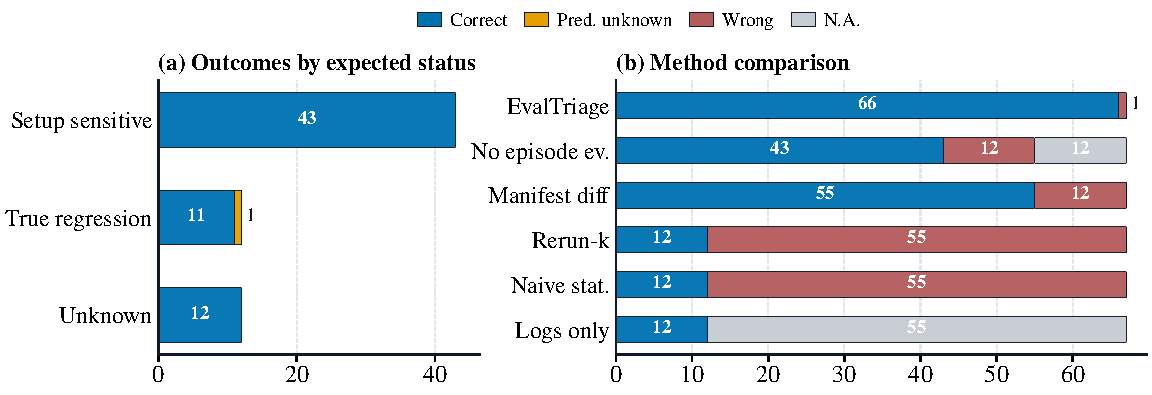
\includegraphics[width=\columnwidth]{figures/rq2_status_overview.pdf}
  \caption{RQ2 status classification: panel (a) shows \sys outcomes by expected status, and panel (b) compares methods by correct, wrong, predicted-unknown, and not-applicable outcomes.}
  \label{fig:rq2-status}
\end{figure}

\subsection{RQ3: Factor Attribution and Abstention}
\label{sub:rq3}

\noindent\textbf{Design.} RQ3 evaluates the central claim of \sys: a deviation diagnosis should connect an observed behavior change to an engineering factor and should abstain when that connection is unsupported. We therefore evaluate completed-rollout and failed-run cases separately. Completed-rollout cases require a thresholded metric or paired-outcome deviation plus replay evidence. Failed-run cases require an execution failure and evidence that the replay or corrected setup recovers execution. Negative calibration cases test the opposite behavior: even if a manifest field differs, \sys should not attribute a factor when no thresholded deviation is detected.

\noindent\textbf{Results.} Table~\ref{tab:paper-results} summarizes the paper-only matrix. Among detected cases, \sys attributes all deviations to the expected factor: 12/12 completed-rollout cases and 4/4 failed-run cases. The combined detected/applicable Top-1 result is therefore 16/16. Under the all-case denominator, the result is 16/20 because the paper-only matrix contains four completed-rollout negative calibration cases where the correct behavior is abstention rather than attribution. The remaining eight negative calibration cases are used only for the robustness/ablation false-attribution denominator. This denominator split is deliberate: detected/applicable Top-1 asks whether \sys identifies the factor when the diagnosis is applicable, while all-case Top-1 keeps abstention cases visible.

\begin{table}[!t]
  \caption{Paper-Only Diagnosis Results}
  \label{tab:paper-results}
  \centering
  \footnotesize
  \renewcommand{\arraystretch}{1.12}
  \begin{tabular}{@{}lrrr@{}}
    \toprule
    Bucket & Detected & Top-1 & All-case \\
    \midrule
    Completed rollout & 75.0\% & 100.0\% & 75.0\% \\
    Failed run & 100.0\% & 100.0\% & 100.0\% \\
    Combined & 80.0\% & 100.0\% & 80.0\% \\
    \bottomrule
  \end{tabular}
\end{table}

\subsection{Ablation and Robustness}
\label{sub:ablation}

\noindent\textbf{Design.} The ablation asks which evidence sources make the attribution reliable. We compare the full method against variants that remove replay evidence, remove episode-level evidence, use manifest differences as a heuristic, use single-run judgment, use a rerun-$k$ style judgment, use a naive statistical gate, or rely on failure-log regexes. These variants are intentionally simple: they represent plausible shortcuts that developers or continuous-integration (CI) systems might use when they do not have factor-directed replay. We recompute the ablation from case artifacts rather than trusting stored baseline summaries, so each method is evaluated under the same artifact contract.

\noindent\textbf{Results.} Table~\ref{tab:ablation} and Figure~\ref{fig:rq3-attribution} summarize the combined robustness ablation. The full method achieves 43/43 detected/applicable Top-1 attribution and 43/55 all-case Top-1, with 0/12 false attributions across the four paper-only and eight robustness-only negative calibration cases. Removing replay lowers detected Top-1 to 38/43. Removing episode evidence lowers the applicable denominator because several completed-rollout cases require paired outcome evidence. The manifest-only heuristic reaches 35/43 detected Top-1 but falsely attributes all 12 negative calibration cases, showing why manifest differences should be treated as suspects rather than causal explanations. The figure also shows the failure anatomy: no-replay misses concentrate in wrong Top-1 factors, no-episode-evidence misses concentrate in no-top-factor outcomes and failed-run non-applicability, and logs-only regex is applicable only to failed runs.

\begin{table}[!t]
  \caption{Combined Ablation Results}
  \label{tab:ablation}
  \centering
  \scriptsize
  \renewcommand{\arraystretch}{1.10}
  \begin{tabular}{@{}lrrr@{}}
    \toprule
    Method & Det. Top-1 & All-case & False attr. \\
    \midrule
    \sys full & 100.0\% & 78.2\% & 0.0\% \\
    No replay & 88.4\% & 69.1\% & 0.0\% \\
    No episode ev. & 64.5\% & 36.4\% & 0.0\% \\
    Manifest diff & 81.4\% & 63.6\% & 100.0\% \\
    Logs only & 100.0\% & 21.8\% & 0.0\% \\
    \bottomrule
  \end{tabular}
\end{table}

\begin{figure}[t]
  \centering
  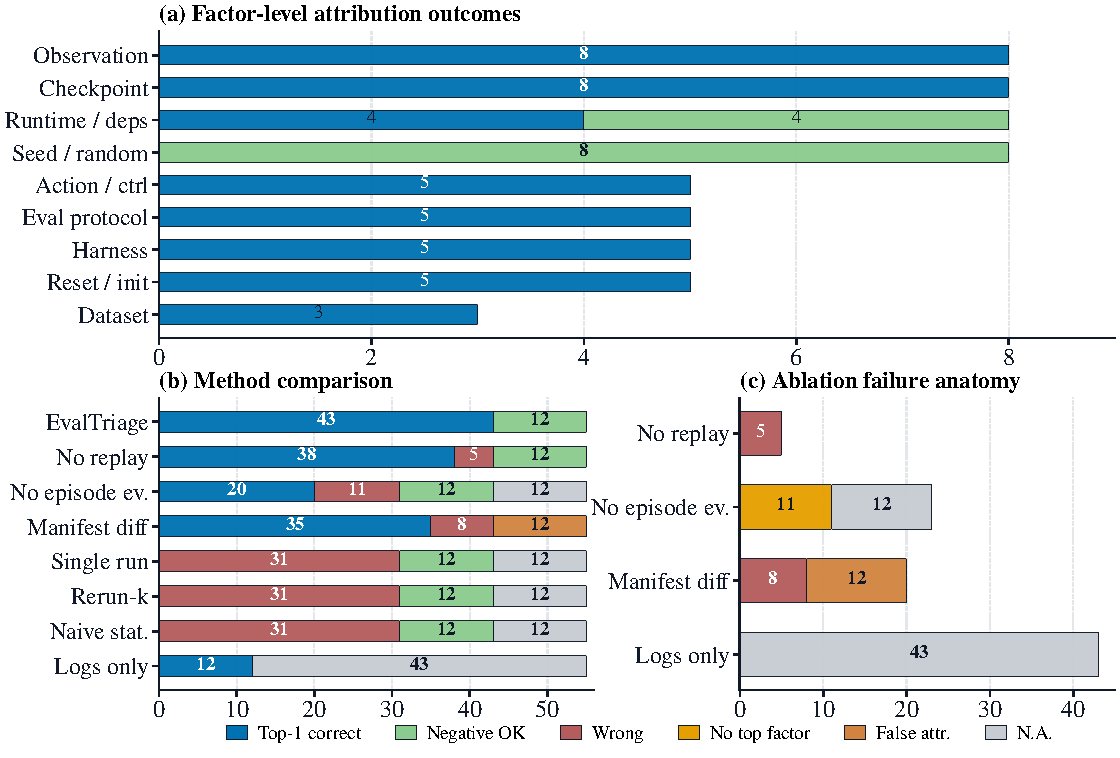
\includegraphics[width=\columnwidth]{figures/rq3_factor_attribution_overview.pdf}
  \caption{RQ3 factor attribution and ablation: panel (a) reports factor-level attribution outcomes, panel (b) compares methods, and panel (c) breaks down ablation failures into wrong, no-top-factor, false-attribution, and not-applicable outcomes.}
  \label{fig:rq3-attribution}
\end{figure}

\subsection{RQ4: Diagnosis Cost}
\label{sub:rq4}

\noindent\textbf{Design.} RQ4 measures the cost of obtaining diagnosis evidence. We report the observed graphics processing unit (GPU) cost of paper-only cases and, for completed-positive cases, the replay workload needed to collect factor-directed evidence. These values are diagnosis-cost measurements for the current artifact pipeline, not claims about model training cost. The key comparison is between affected-task replay, a full single replay, and a blind rerun-$k$ baseline with $k=3$.

\begin{figure}[t]
  \centering
  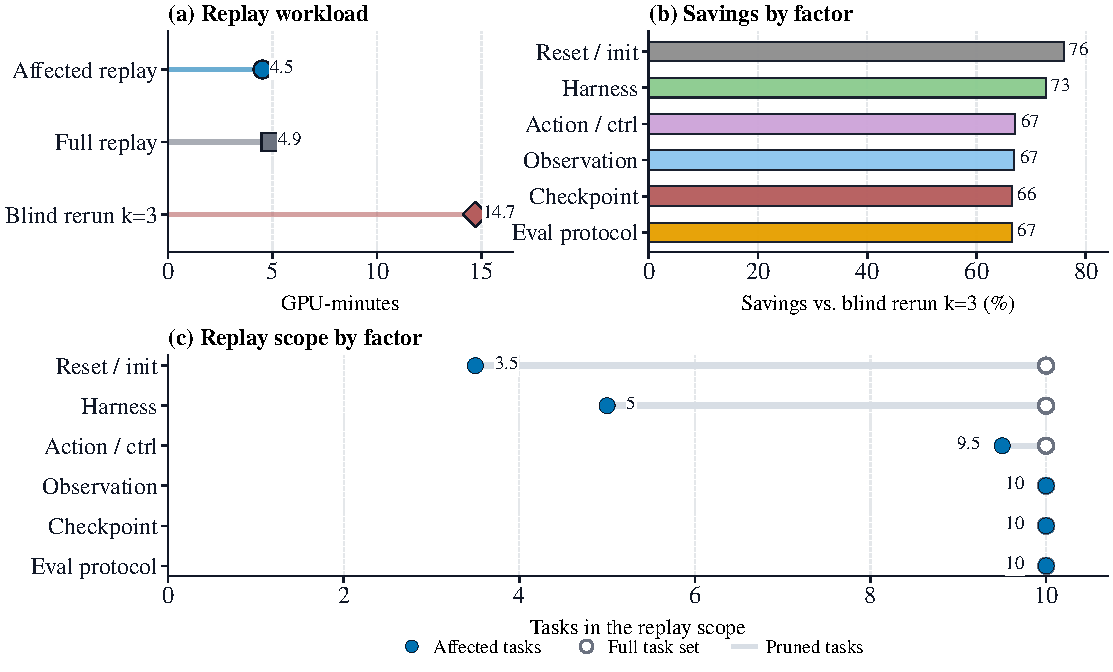
\includegraphics[width=\columnwidth]{figures/rq4_cost_overview.pdf}
  \caption{RQ4 diagnosis cost: panel (a) compares replay workloads, panel (b) reports savings over blind rerun-$k$, and panel (c) shows how affected-task replay prunes the task scope by factor.}
  \label{fig:rq4-cost}
\end{figure}

\noindent\textbf{Results.} Table~\ref{tab:cost} summarizes paper-only cost measurements, and Figure~\ref{fig:rq4-cost} shows the replay-workload comparison. Completed-positive cases average 15.41 observed GPU-minutes and 22.89 wall-clock minutes per case. Their measured affected-task replay averages 4.52 GPU-minutes, close to a full single replay when the affected task set spans most tasks, but far below the 14.71 GPU-minutes of a blind rerun-$k$ baseline. Savings against blind rerun-$k$ range from 66\% to 76\% across factor buckets. The largest replay-scope reductions occur for reset/initial-state and harness cases, where the affected task sets average 3.5 and 5.0 tasks out of 10 respectively. Failed-run cases are cheaper to observe on average because the current run fails early, but they still require recovery evidence before attribution.

\begin{table}[!t]
  \caption{Paper-Only Diagnosis Cost}
  \label{tab:cost}
  \centering
  \scriptsize
  \renewcommand{\arraystretch}{1.10}
  \begin{tabular}{@{}lrrrr@{}}
    \toprule
    Bucket & N & Obs. GPU & Obs. wall & Aff. GPU \\
    \midrule
    Comp. positive & 12 & 15.41 & 22.89 & 4.52 \\
    Comp. negative & 4 & 14.79 & 19.95 & -- \\
    Failed run & 4 & 5.22 & 8.05 & -- \\
    All paper & 20 & 13.25 & 19.34 & -- \\
    \bottomrule
  \end{tabular}
  \vspace{1pt}
  \parbox{0.96\columnwidth}{\scriptsize GPU/wall values are minutes. Aff. GPU is measured for the 12 completed-positive cases where affected-task replay is meaningful.}
\end{table}
